\section{Câu 8}
Cho một tín hiệu cần xử lý dưới dạng dòng điện, có tầm thay đổi từ 1mA -- 10mA.

a. Thiết kế mạch cho ngõ ra tầm 0V -- 5V.

b. Lựa chọn OPAMP và các linh kiện cần thiết để mạch hoạt động. Lưu ý: xử lý các
thông số không lý tưởng của OPAMP. (Tham khảo datasheet)

\begin{center}
\textbf{Bài giải}
\end{center}

a. Để thiết kế mạch chuyển đổi tín hiệu dòng điện sang điện áp ta biểu diễn mối quan hệ giữa dòng điện và điện áp như hình bên dưới
\begin{figure}[H]
    \centering
    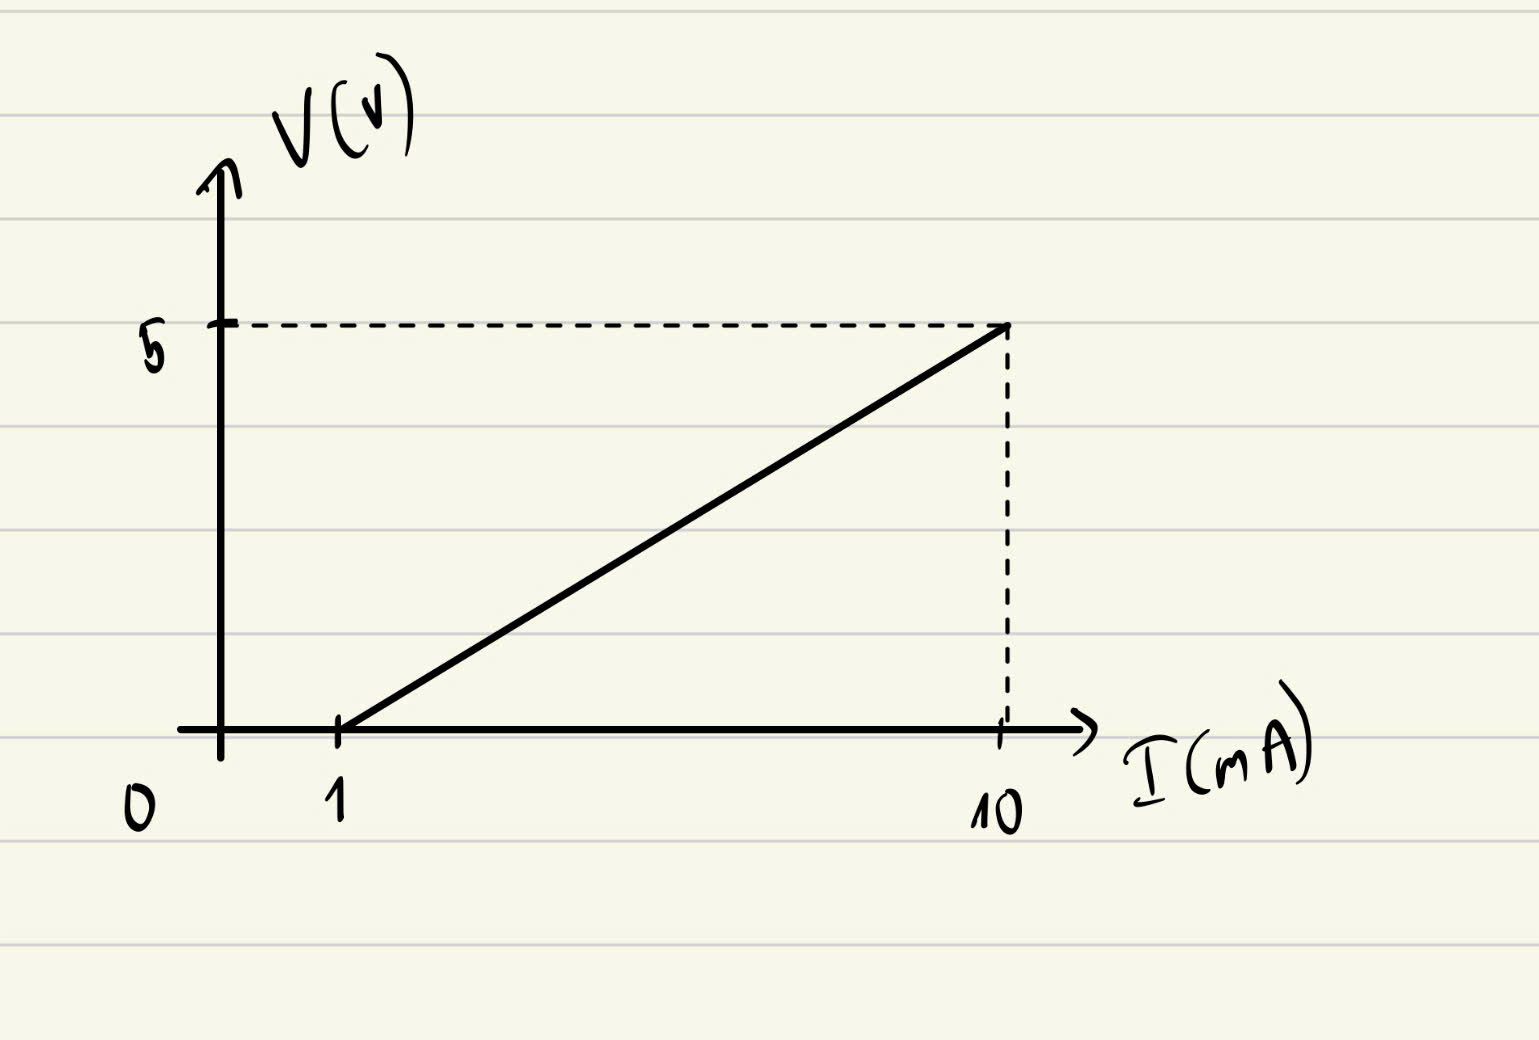
\includegraphics[scale=0.2]{image/C8_chart.png} 
\end{figure}
Từ hình trên ta có hệ phương trình:
\begin{equation*}
    \begin{cases}
        0 = 1\cdot a + b  \\
        5 = 10\cdot a + b\\
    \end{cases}
\end{equation*}
Giải hệ phương trình ta được:  
\begin{equation*}
    \begin{cases}
        a = \dfrac{5}{9} \\
        b = -\dfrac{5}{9} \\
    \end{cases}
\end{equation*}
Vậy ta có phương trình mạch chuyển đổi dòng điện sang điện áp như sau:
\begin{equation*}
    \boxed{V = \dfrac{5}{9}I + \dfrac{5}{9}}
\end{equation*}
\textbf{b.} Thiết kế mạch

Từ phương trình trên
Dùng 1 OPAMP (OPA2333) để làm mạch đảo pha điện áp 5/9 thành điện áp -5/9V.

Dùng 1 OPAMP (LM358P) chuyển đổi dòng thành áp theo tỉ lệ 5/9 V/mA.

Dùng 1 OPAMP (OPA233) cộng 2 điện áp lại với nhau.
Ở mạch U2A, dùng mạch chia áp với nguồn 5.5V để tạo điện áp tham chiếu ngõ vào là $\dfrac{5}{9}V$. Chọn các điện trở:
\begin{equation*}
    R_9 = 760\,\Omega,\quad R_{10} = 100\,\Omega
\end{equation*}


Việc chọn giá trị điện trở được thực hiện như sau:
\begin{itemize}
    \item Các điện trở R$_1$, R$_3$, R$_4$, R$_5$ trong mạch khuếch đại chọn bằng 560\,$\Omega$ để đảm bảo tỉ lệ khuếch đại.
    \item Các điện trở phân cực và hồi tiếp khác chọn giá trị $560\,\Omega$ để giảm thiểu ảnh hưởng của dòng bias.
\end{itemize}
Chọn OPAMP LM358P vì các thông số tham khảo được:
\begin{itemize}
    \item Vsupply : 3V -- 32V, phù hợp với nguồn cấp phổ biến.
    \item Vos (độ dịch chuyển ngõ vào): 2mV.
    \item Ib (dòng dịch chuyển ngõ vào): 2nA.
    \item Ios (dòng dịch chuyển bù ngõ vào): 20nA (max).
\end{itemize}
Chọn OPAMP OPA2333 vì các thông số tham khảo được:
\begin{itemize}
    \item Khả năng rail to rail ở ngõ ra: có.
    \item Vos (độ dịch chuyển ngõ vào): 2$\mu $V.
    \item Ib (dòng dịch chuyển ngõ vào): 2pA.
    \item Ios (dòng dịch chuyển bù ngõ vào): 140pA.
    \item Các sai số ngõ vào rất bé nhưng nguồn cấp khá nhỏ.
\end{itemize}
Mạch hoàn chỉnh như hình bên dưới:
\begin{figure}[H]
    \centering
    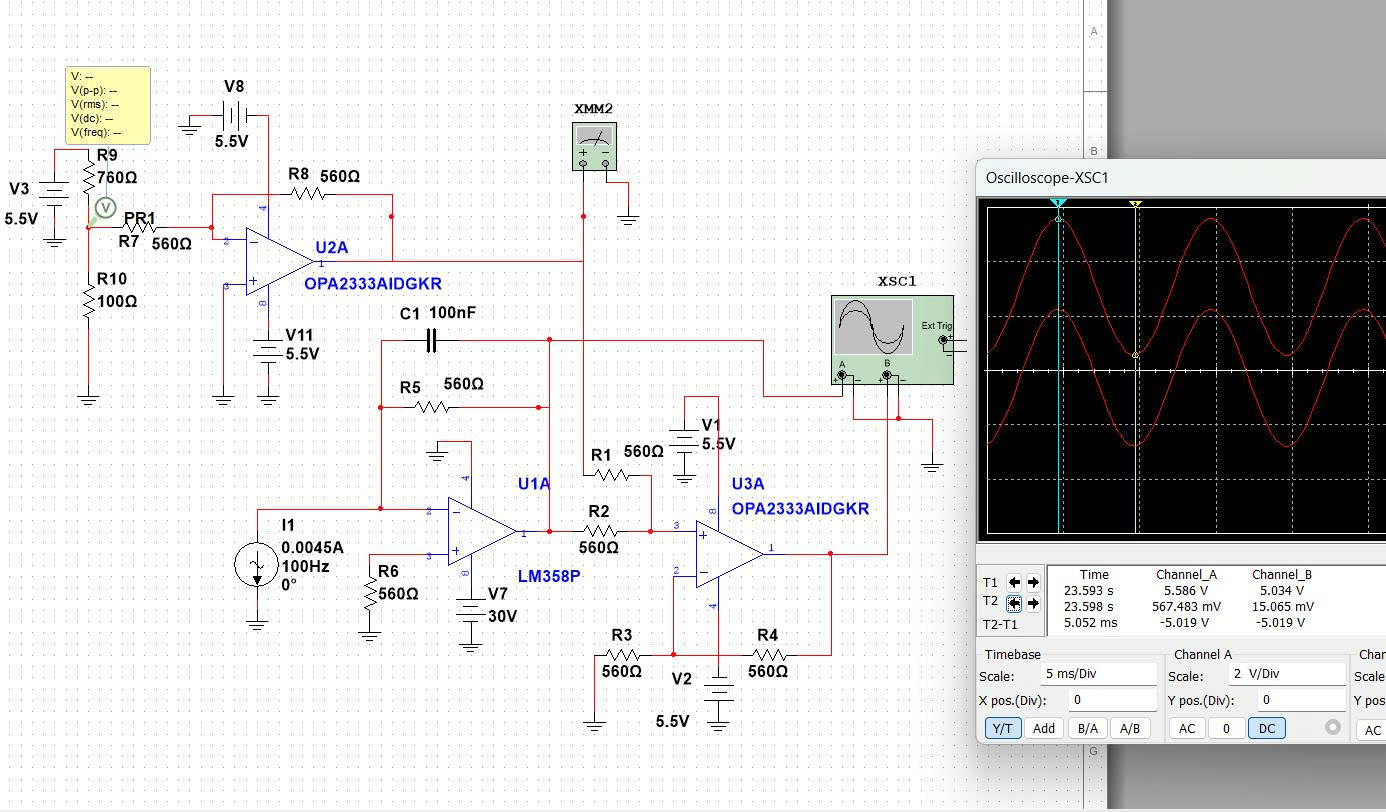
\includegraphics[scale=0.32]{image/C8.png}
\end{figure}